\documentclass[a4paper,twocolumn,10pt,margin=0.5in]{extreport}

%\usepackage{concmath}
\usepackage{tgschola}
\usepackage[margin=1in]{geometry}
\usepackage[utf8]{inputenc}
\usepackage[T1]{fontenc}
\usepackage{mathrsfs}
\usepackage{textcomp}
\usepackage[french]{babel}
\usepackage{amsmath}
\usepackage{amssymb}
\usepackage{cancel}
\usepackage{frcursive}
\usepackage[inline]{asymptote}
\usepackage{tikz}
\usepackage[european,straightvoltages,europeanresistors]{circuitikz}
\usepackage{tikz-cd}
\usepackage{tkz-tab}
\usepackage[b]{esvect}
\usepackage[framemethod=TikZ]{mdframed}
\usepackage{centernot}
\usepackage{diagbox}
\usepackage{dsfont}
\usepackage{fancyhdr}
\usepackage{float}
\usepackage{graphicx}
\usepackage{listings}
\usepackage{multicol}
\usepackage{nicematrix}
\usepackage{pdflscape}
\usepackage{stmaryrd}
\usepackage{xfrac}
\usepackage{hep-math-font}
\usepackage{amsthm}
\usepackage{thmtools}
\usepackage{indentfirst}
\usepackage[framemethod=TikZ]{mdframed}
\usepackage{accents}
\usepackage{soulutf8}
\usepackage{mathtools}
\usepackage{bodegraph}
\usepackage{slashbox}
\usepackage{enumitem}
\usepackage{calligra}
\usepackage{cinzel}
\usepackage{BOONDOX-calo}

% Tikz
\usetikzlibrary{babel}
\usetikzlibrary{positioning}
\usetikzlibrary{calc}

% global settings
\frenchspacing
\reversemarginpar
\setuldepth{a}

%\everymath{\displaystyle}

\frenchbsetup{StandardLists=true}

\def\asydir{asy}

%\sisetup{exponent-product=\cdot,output-decimal-marker={,},separate-uncertainty,range-phrase=\;à\;,locale=FR}

\setlength{\parskip}{1em}

\theoremstyle{definition}

% Changing math
\let\emptyset\varnothing
\let\ge\geqslant
\let\le\leqslant
\let\preceq\preccurlyeq
\let\succeq\succcurlyeq
\let\ds\displaystyle
\let\ts\textstyle

\newcommand{\C}{\mathds{C}}
\newcommand{\R}{\mathds{R}}
\newcommand{\Z}{\mathds{Z}}
\newcommand{\N}{\mathds{N}}
\newcommand{\Q}{\mathds{Q}}

\renewcommand{\O}{\emptyset}

\newcommand\ubar[1]{\underaccent{\bar}{#1}}

\renewcommand\Re{\expandafter\mathfrak{Re}}
\renewcommand\Im{\expandafter\mathfrak{Im}}

\let\slantedpartial\partial
\DeclareRobustCommand{\partial}{\text{\rotatebox[origin=t]{20}{\scalebox{0.95}[1]{$\slantedpartial$}}}\hspace{-1pt}}

% merging two maths characters w/ \charfusion
\makeatletter
\def\moverlay{\mathpalette\mov@rlay}
\def\mov@rlay#1#2{\leavevmode\vtop{%
   \baselineskip\z@skip \lineskiplimit-\maxdimen
   \ialign{\hfil$\m@th#1##$\hfil\cr#2\crcr}}}
\newcommand{\charfusion}[3][\mathord]{
    #1{\ifx#1\mathop\vphantom{#2}\fi
        \mathpalette\mov@rlay{#2\cr#3}
      }
    \ifx#1\mathop\expandafter\displaylimits\fi}
\makeatother

% custom math commands
\newcommand{\T}{{\!\!\,\top}}
\newcommand{\avrt}[1]{\rotatebox{-90}{$#1$}}
\newcommand{\bigcupdot}{\charfusion[\mathop]{\bigcup}{\cdot}}
\newcommand{\cupdot}{\charfusion[\mathbin]{\cup}{\cdot}}
%\newcommand{\danger}{{\large\fontencoding{U}\fontfamily{futs}\selectfont\char 66\relax}\;}
\newcommand{\tendsto}[1]{\xrightarrow[#1]{}}
\newcommand{\vrt}[1]{\rotatebox{90}{$#1$}}
\newcommand{\tsup}[1]{\textsuperscript{\underline{#1}}}
\newcommand{\tsub}[1]{\textsubscript{#1}}

\renewcommand{\mod}[1]{~\left[ #1 \right]}
\renewcommand{\t}{{}^t\!}
\newcommand{\s}{\text{\calligra s}}

% custom units / constants
%\DeclareSIUnit{\litre}{\ell}
\let\hbar\hslash

% header / footer
\pagestyle{fancy}
\fancyhead{} \fancyfoot{}
\fancyfoot[C]{\thepage}

% fonts
\let\sc\scshape
\let\bf\bfseries
\let\it\itshape
\let\sl\slshape

% custom math operators
\let\th\relax
\let\det\relax
\DeclareMathOperator*{\codim}{codim}
\DeclareMathOperator*{\dom}{dom}
\DeclareMathOperator*{\gO}{O}
\DeclareMathOperator*{\po}{\text{\cursive o}}
\DeclareMathOperator*{\sgn}{sgn}
\DeclareMathOperator*{\simi}{\sim}
\DeclareMathOperator{\Arccos}{Arccos}
\DeclareMathOperator{\Arcsin}{Arcsin}
\DeclareMathOperator{\Arctan}{Arctan}
\DeclareMathOperator{\Argsh}{Argsh}
\DeclareMathOperator{\Arg}{Arg}
\DeclareMathOperator{\Aut}{Aut}
\DeclareMathOperator{\Card}{Card}
\DeclareMathOperator{\Cl}{\mathcal{C}\!\ell}
\DeclareMathOperator{\Cov}{Cov}
\DeclareMathOperator{\Ker}{Ker}
\DeclareMathOperator{\Mat}{Mat}
\DeclareMathOperator{\PGCD}{PGCD}
\DeclareMathOperator{\PPCM}{PPCM}
\DeclareMathOperator{\Supp}{Supp}
\DeclareMathOperator{\Vect}{Vect}
\DeclareMathOperator{\argmax}{argmax}
\DeclareMathOperator{\argmin}{argmin}
\DeclareMathOperator{\ch}{ch}
\DeclareMathOperator{\com}{com}
\DeclareMathOperator{\cotan}{cotan}
\DeclareMathOperator{\det}{det}
\DeclareMathOperator{\id}{id}
\DeclareMathOperator{\rg}{rg}
\DeclareMathOperator{\rk}{rk}
\DeclareMathOperator{\sh}{sh}
\DeclareMathOperator{\th}{th}
\DeclareMathOperator{\tr}{tr}

% colors and page style
\definecolor{truewhite}{HTML}{ffffff}
\definecolor{white}{HTML}{faf4ed}
\definecolor{trueblack}{HTML}{000000}
\definecolor{black}{HTML}{575279}
\definecolor{mauve}{HTML}{907aa9}
\definecolor{blue}{HTML}{286983}
\definecolor{red}{HTML}{d7827e}
\definecolor{yellow}{HTML}{ea9d34}
\definecolor{gray}{HTML}{9893a5}
\definecolor{grey}{HTML}{9893a5}
\definecolor{green}{HTML}{a0d971}

\pagecolor{white}
\color{black}

\begin{asydef}
	settings.prc = false;
	settings.render=0;

	white = rgb("faf4ed");
	black = rgb("575279");
	blue = rgb("286983");
	red = rgb("d7827e");
	yellow = rgb("f6c177");
	orange = rgb("ea9d34");
	gray = rgb("9893a5");
	grey = rgb("9893a5");
	deepcyan = rgb("56949f");
	pink = rgb("b4637a");
	magenta = rgb("eb6f92");
	green = rgb("a0d971");
	purple = rgb("907aa9");

	defaultpen(black + fontsize(8pt));

	import three;
	currentlight = nolight;
\end{asydef}

% theorems, proofs, ...

\mdfsetup{skipabove=1em,skipbelow=1em, innertopmargin=6pt, innerbottommargin=6pt,}

\declaretheoremstyle[
	headfont=\normalfont\itshape,
	numbered=no,
	postheadspace=\newline,
	headpunct={:},
	qed=\qedsymbol]{demstyle}

\declaretheorem[style=demstyle, name=Démonstration]{dem}

\newcommand\veczero{\kern-1.2pt\vec{\kern1.2pt 0}} % \vec{0} looks weird since the `0' isn't italicized

\makeatletter
\renewcommand{\title}[2]{
	\AtBeginDocument{
		\begin{titlepage}
			\begin{center}
				\vspace{10cm}
				{\Large \sc Chapitre #1}\\
				\vspace{1cm}
				{\Huge \calligra #2}\\
				\vfill
				Hugo {\sc Salou} MPI${}^{\star}$\\
				{\small Dernière mise à jour le \@date }
			\end{center}
		\end{titlepage}
	}
}

\newcommand{\titletp}[4]{
	\AtBeginDocument{
		\begin{titlepage}
			\begin{center}
				\vspace{10cm}
				{\Large \sc tp #1}\\
				\vspace{1cm}
				{\Huge \textsc{\textit{#2}}}\\
				\vfill
				{#3}\textit{MPI}${}^{\star}$\\
			\end{center}
		\end{titlepage}
	}
	\fancyfoot{}\fancyhead{}
	\fancyfoot[R]{#4 \textit{MPI}${}^{\star}$}
	\fancyhead[C]{{\sc tp #1} : #2}
	\fancyhead[R]{\thepage}
}

\newcommand{\titletd}[2]{
	\AtBeginDocument{
		\begin{titlepage}
			\begin{center}
				\vspace{10cm}
				{\Large \sc td #1}\\
				\vspace{1cm}
				{\Huge \calligra #2}\\
				\vfill
				Hugo {\sc Salou} MPI${}^{\star}$\\
				{\small Dernière mise à jour le \@date }
			\end{center}
		\end{titlepage}
	}
}
\makeatother

\newcommand{\sign}{
	\null
	\vfill
	\begin{center}
		{
			\fontfamily{ccr}\selectfont
			\textit{\textbf{\.{\"i}}}
		}
	\end{center}
	\vfill
	\null
}

\renewcommand{\thefootnote}{\emph{\alph{footnote}}}

% figure support
\usepackage{import}
\usepackage{xifthen}
\pdfminorversion=7
\usepackage{pdfpages}
\usepackage{transparent}
\newcommand{\incfig}[1]{%
	\def\svgwidth{\columnwidth}
	\import{./figures/}{#1.pdf_tex}
}

\pdfsuppresswarningpagegroup=1
\ctikzset{tripoles/european not symbol=circle}

\newcommand{\missingpart}{{\large\color{red} Il manque quelque chose ici\ldots}}

\usepackage{caption}
\usepackage{subcaption}
\usepackage{comment}
\usepackage{pgfornament}
\usepackage{graphicx}
\usepackage{pgfplots}
\usepackage{multirow}

%\begin{comment}

\definecolor{black}{HTML}{000000}
\definecolor{white}{HTML}{ffffff}
\color{black}
\pagecolor{white}

\begin{asydef}
	white = rgb("ffffff");
	black = rgb("000000");
	defaultpen(black + fontsize(8pt));
\end{asydef}
%\end{comment}

\definecolor{BleuClair}{HTML}{286983}
\definecolor{LightBlue}{cmyk}{0.22,0.05,0,0.1}
\definecolor{GrisClair}{HTML}{9893a5}
\def\res#1{{\color{cyan}#1}}

\titletp{o\:3}{Étude des ondes électromagnétiques centimétriques}{\begin{tabular}{c}Hugo \textsc{Salou}\\Noémie \textsc{Combey}\end{tabular}}{Hugo \textsc{Salou} \& Noémie \textsc{Combey}}

\def\thesection{\Roman{section}.}
\def\thesubsection{\Roman{section}.\Alph{subsection}.}

\begin{document}
	L'objectif de ce \textsc{tp} est la détection et l'analyse d'ondes centimétriques.
	On étudiera notamment leur polarisation, et la formation d'interférences.

	\bigskip

	\section{Pénétration dans le bois et le métal}

	On commence par s'intéresser à la transparence du bois et du métal pour des ondes électromagnétiques dans le domaine centimétrique.
	On réalise le montage représenté sur la figure~\ref{fig:montage-transparence} : on place entre émetteur et récepteur une plaque en bois. Par la suite, on remplacera la plaque de bois par une plaque en métal.
		
	\begin{figure}[H]
		\centering
		\vspace{-1cm}
		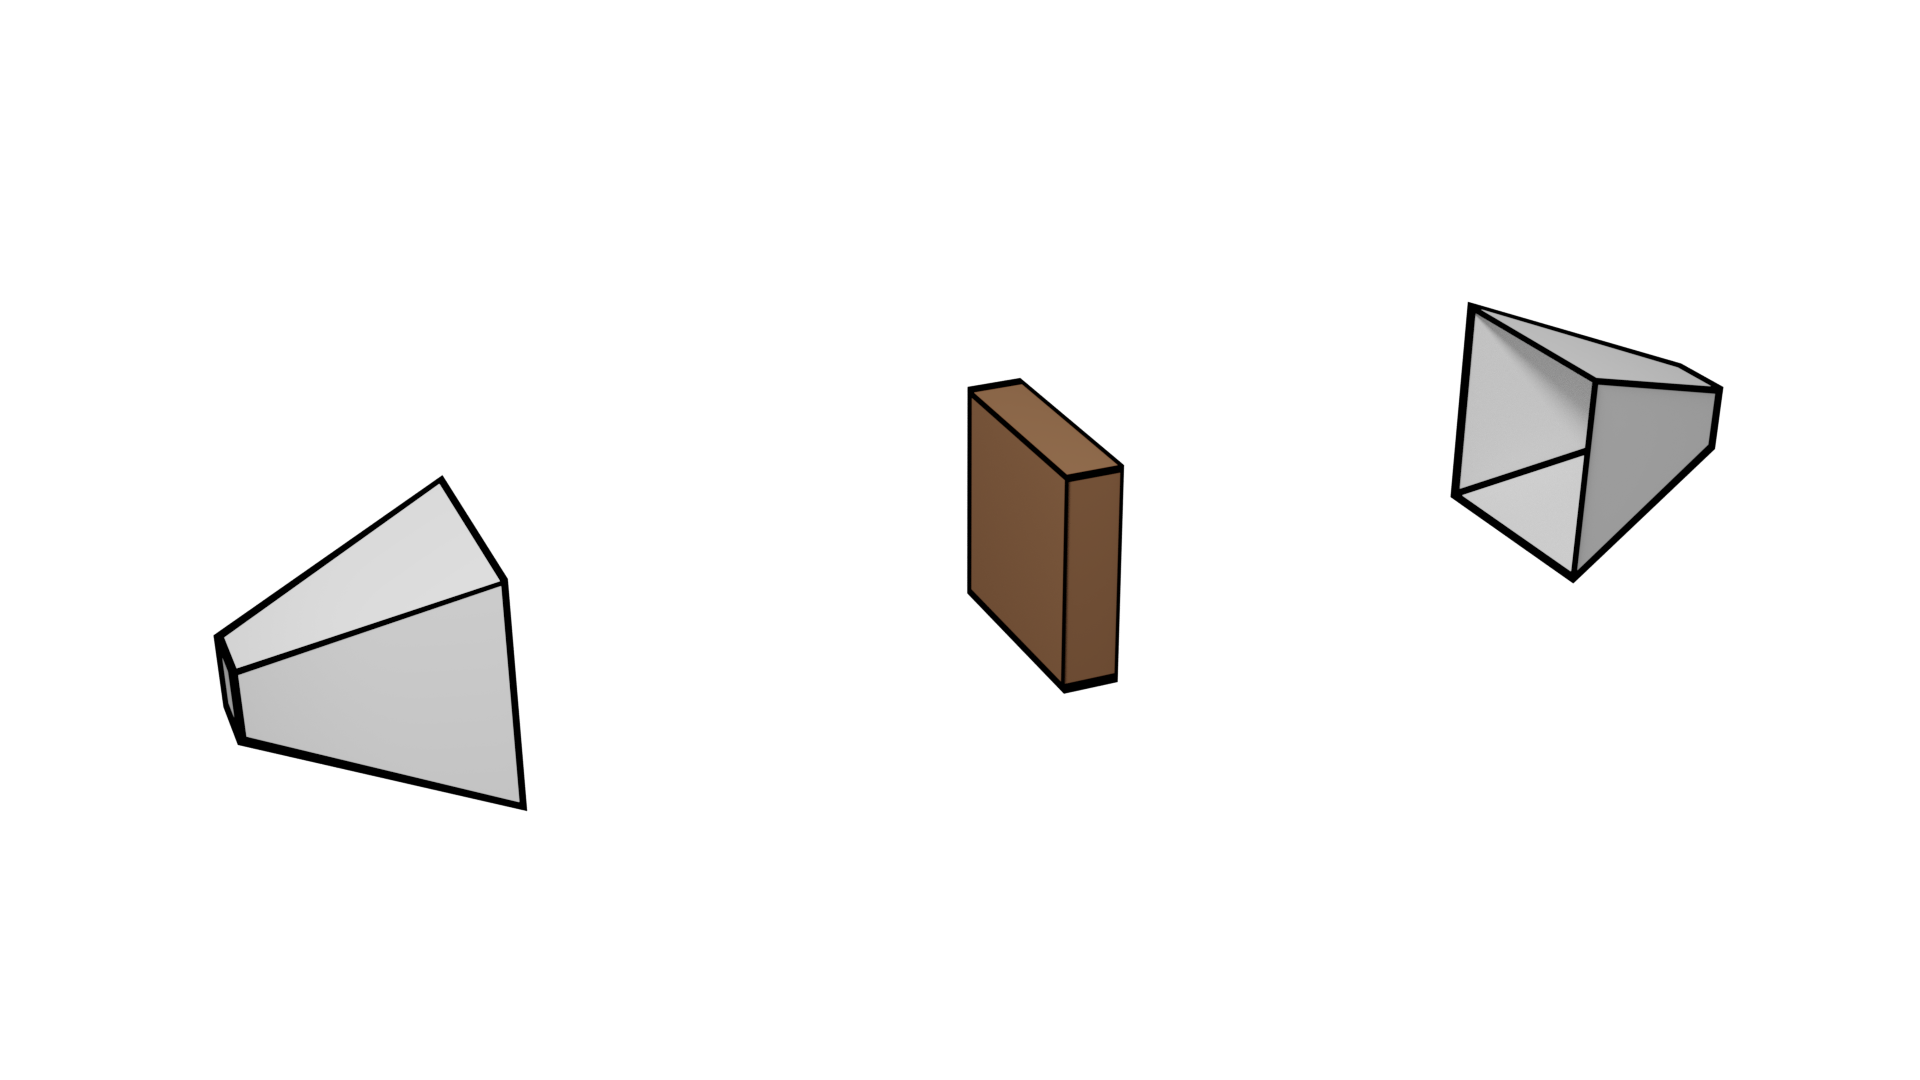
\includegraphics[width=\linewidth]{figures/montage-1.png}
		\vspace{-1cm}
		\caption{Montage pour la mesure de pénétration dans le bois et le métal}
		\label{fig:montage-transparence}
	\end{figure}

	On émet une onde centimétrique de fréquence~$f = 9{,}5\:\mathrm{GHz}$, et on mesure le signal reçu à l'aide d'un oscilloscope.
	En particulier, on mesure l'amplitude du signal.
	Pour la plaque en bois, on mesure une amplitude de \res{$A_{\mathrm{bois}} \simeq 8{,}8\:\mathrm{V}$}.
	On remplace la plaque en bois par celle en métal, et on mesure une amplitude de \res{$A_{\mathrm{m\acute{e}tal}} \simeq 100\:\mathrm{mV}$}.
	Finalement, on retire la plaque en métal, et on mesure l'amplitude reçue : \res{$A_\mathrm{vide} \simeq 10{,}3 \:\mathrm{V}$}.

	Le bois est transparent aux ondes centimétriques, et le métal est opaque.

	\bigskip

	\section{Polarisation des ondes}

	L'onde émise est polarisée rectilignement. En effet, en faisant tourner l'émetteur par rapport au récepteur, on observe que l'amplitude est presque nulle lorsque l'angle relatif entre l'émetteur et le récepteur est à $90\:^\circ$.
	Afin de mesurer la direction de polarisation, on place une grille de polarisation dans le montage, comme montré sur la figure~\ref{fig:montage-polarisation}.

	\begin{figure}[H]
		\centering
		\vspace{-1cm}
		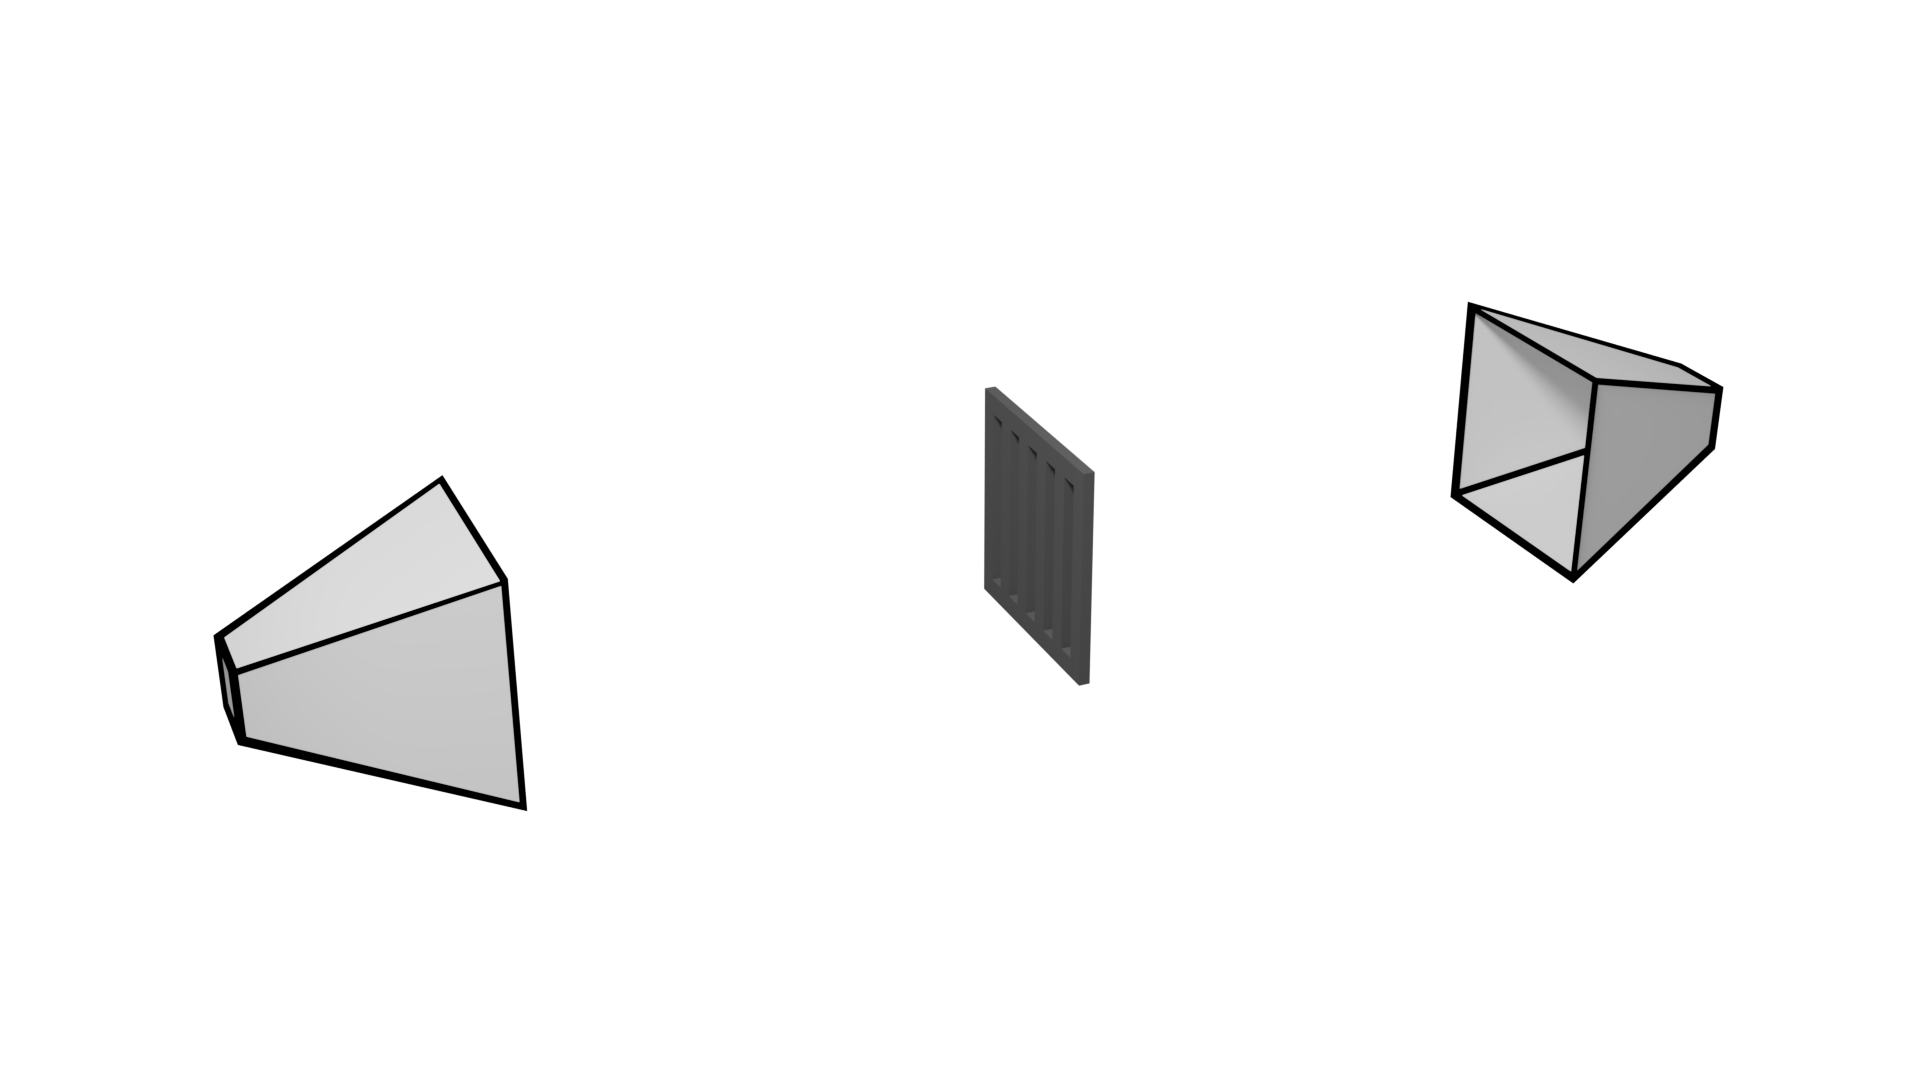
\includegraphics[width=\linewidth]{figures/montage-2.png}
		\vspace{-1cm}
		\caption{Montage pour la mesure de polarisation dans le bois et le métal}
		\label{fig:montage-polarisation}
	\end{figure}

	On peut remarquer que l'onde est bloquée lorsque la grille de polarisation est horizontale, mais ne l'est pas lorsque la grille de polarisation est verticale.
	On représente le champ $\vec{E}(\mathrm{M})$ pour les deux orientations de la grille sur la figure~\ref{fig:montage-polarisation-champs}.

	\begin{figure}[H]
		\centering
		\vspace{-1cm}
		\subcaptionbox{Grille verticale}{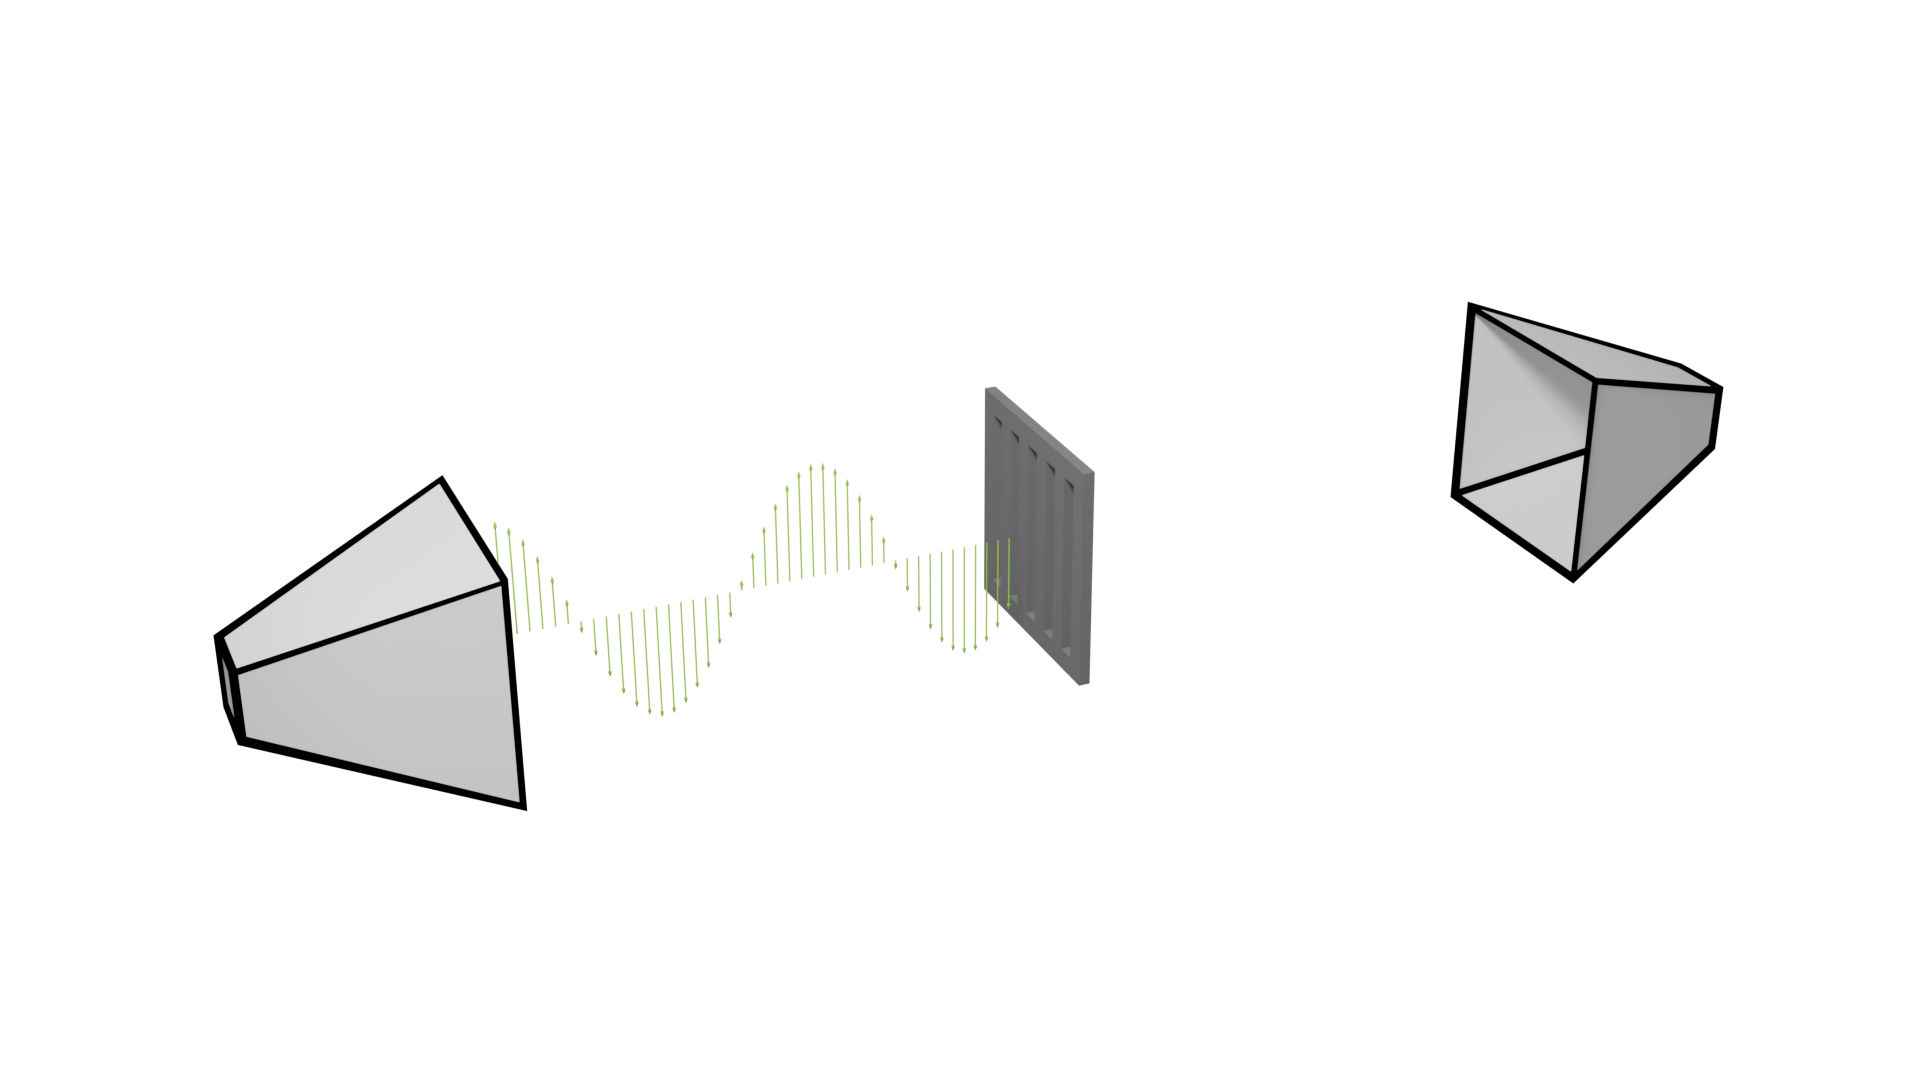
\includegraphics[width=\linewidth]{figures/montage-2a.png}\vspace{-1cm}}
		\vspace{-1cm}
		\subcaptionbox{Grille horizontale}{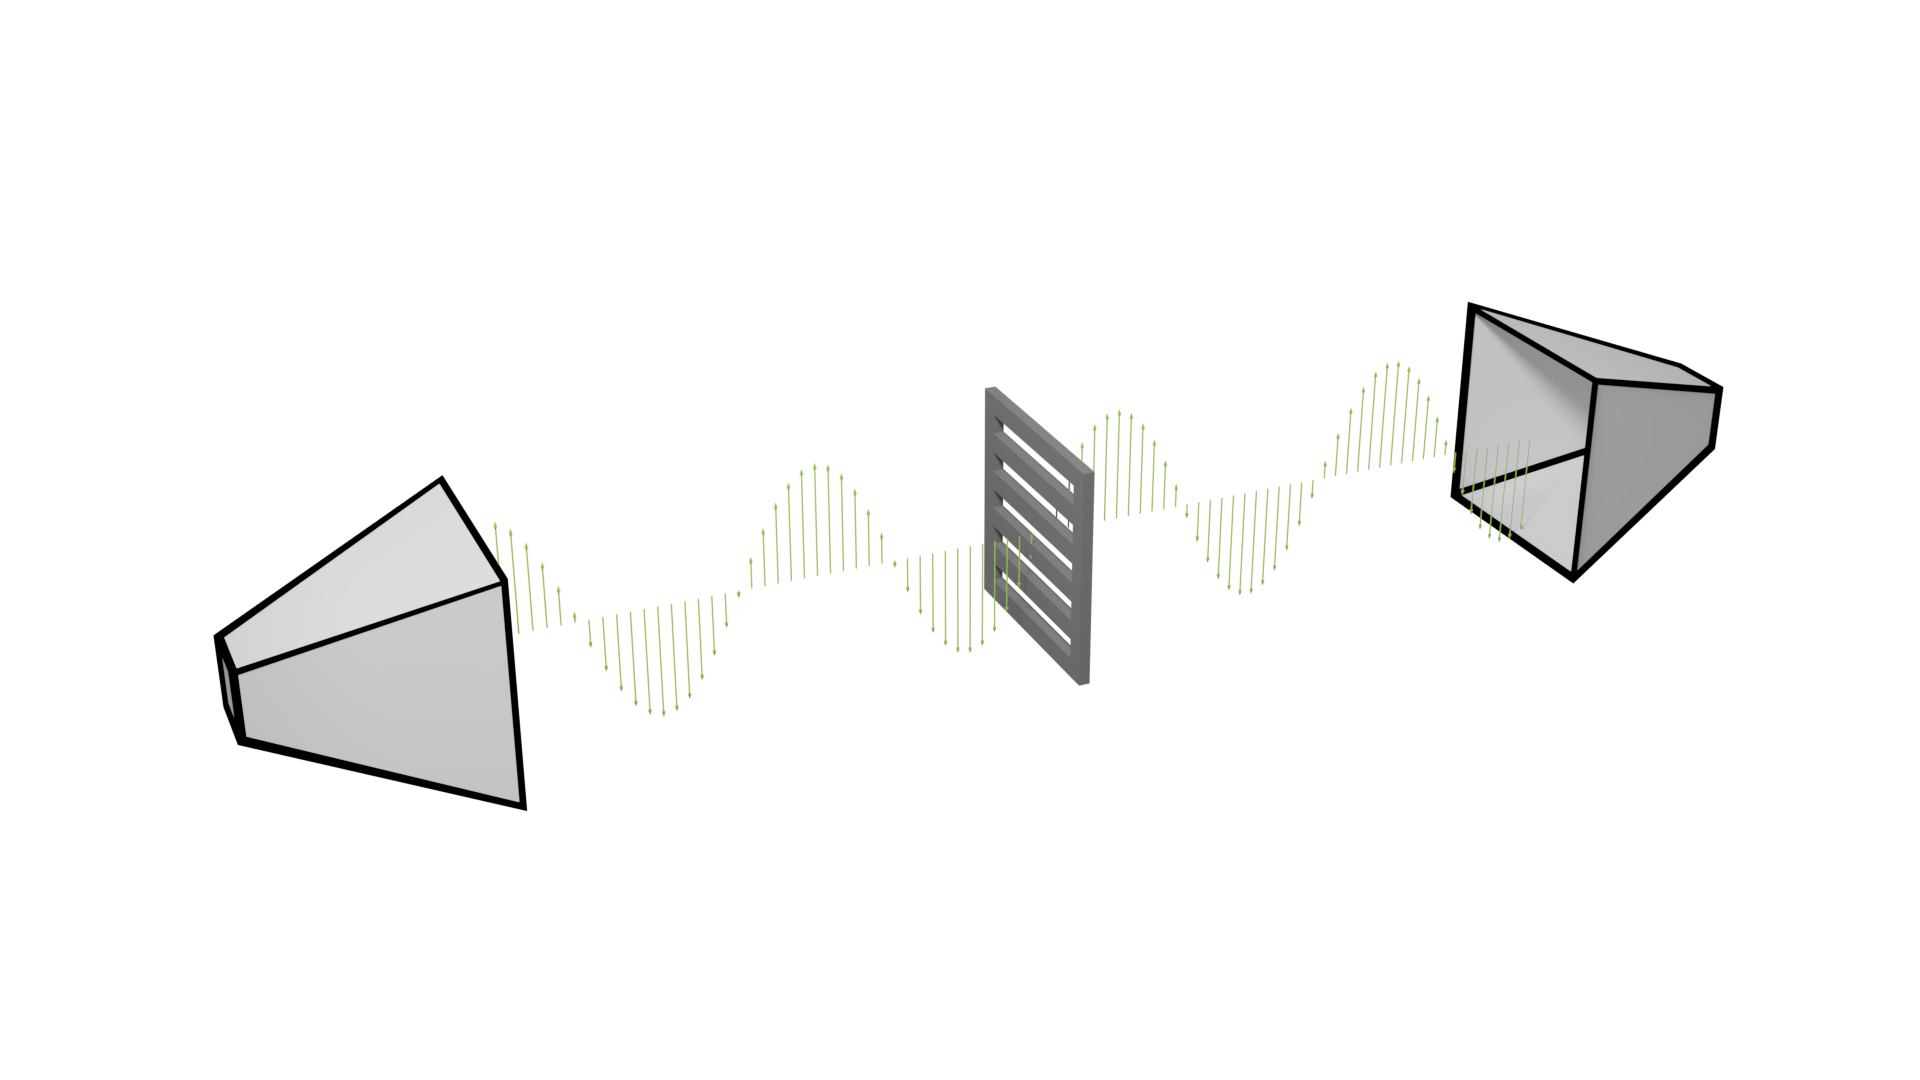
\includegraphics[width=\linewidth]{figures/montage-2b.png}\vspace{-1cm}}
		\vspace{1cm}
		\caption{Champ $\vec{E}(\mathrm{M})$, passage ou non de l'onde en fonction de l'orientation de la grille}
		\label{fig:montage-polarisation-champs}
	\end{figure}

	\bigskip

	\section{Ondes stationnaires}

	On cherche, à présent, à mesurer la longueur d'onde $\lambda_0$ de l'onde centimétrique émise.
	On place une plaque métallique en sortie de l'émetteur d'ondes centimétriques, et on déplace une sonde \guillemotleft~sans cornet~\guillemotright\ entre l'émetteur et la plaque.

	L'onde émise est réfléchie sur la plaque métallique, ce qui entraine l'apparition d'une onde stationnaire.
	En observant le signal reçu par l'antenne, on cherche un nœud du champ $\vec{E}(\mathrm{M})$, et on note la coordonnée $x$ de ce point.
	Une fois trouvé, on cherche le nœud suivant, et on note la coordonnée $x'$ de ce point.
	Entre un nœud et le suivant, la distance est de $\lambda_0 / 2$, comme le montre la figure~\ref{fig:onde-stationnaire}.

	\begin{figure}[H]
		\centering
		\begin{asy}
			import graph;

			size(8cm);

			real k = 1.5;

			real f(real x) { return 3*sin((x-k)/2); }
			real g(real x) { return -3*sin((x-k)/2); }

			draw(graph(f, -10, 10), red);
			draw(graph(g, -10, 10), red);

			draw((-11,0)--(11,0), Arrow(TeXHead));
			draw((0,-4)--(0,4), Arrow(TeXHead));

			draw((k,0)--(k,-4), dashed);
			draw((k+2pi,0)--(k+2pi,-4), dashed);
			draw((k+2pi,-4)--(k,-4), Arrows(TeXHead));
			label("$\ds\frac{\lambda_0}{2}$", (k+pi,-4), align=S);
			label("$x$", (11,0), align=SE);
			label("$\vec{E}(x) \cdot \vec{e}_z$", (0, 4), align=NW);
		\end{asy}
		\caption{Onde stationnaire et distance entre deux nœuds}
		\label{fig:onde-stationnaire}
	\end{figure}

	On réalise le protocole décrit, et on mesure la distance entre 5 nœuds : \res{$\mathrm{\Delta}x = 80\:\mathrm{mm}$}.
	On en déduit la valeur de la longueur d'onde $\lambda_0$ : \[
		\res{\lambda_0 = 3{,}2\:\mathrm{cm}}
	,\] valeur qui est cohérente avec celle donnée dans l'énoncé : $\lambda_0 = 3{,}16\:\mathrm{cm}$.

	\bigskip

	\section{Interféromètre de \textsc{Michelson}}

	On réalise un interféromètre de \textsc{Michelson} pour les ondes centimétriques.
	On utilise donc des plaques en métal comme miroirs, et la plaque de bois comme séparatrice.
	Le montage est représenté sur la figure~\ref{fig:montage-michelson}.

	\begin{figure}[H]
		\centering
		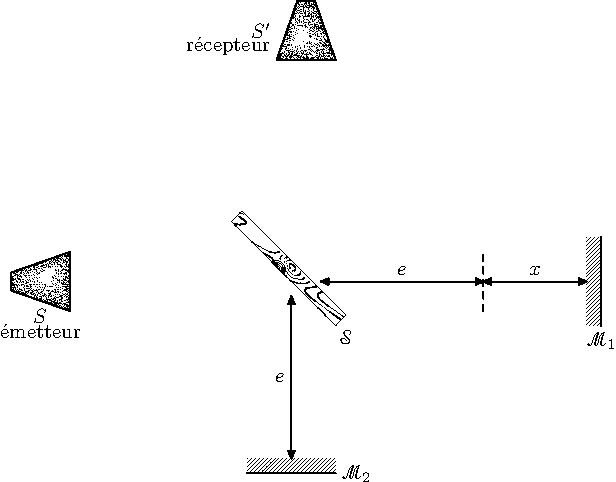
\includegraphics[width=\linewidth]{figures/michelson-1.pdf}
		\caption{Interféromètre de \textsc{Michelson} à onde centimétriques}
		\label{fig:montage-michelson}
	\end{figure}

	On règle le Michelson en lame d'air.
	Ainsi, la différence de marche $\delta(\mathrm{M})$ est donnée par la formule $2\,n_\mathrm{air}\,e\,\cos i$, où $e$ les l'épaisseur de la lame d'air, et $i$ est l'angle entre la normale à \guillemotleft~l'écran,~\guillemotright\ et le point $\mathrm{M}$.
	En alignant le récepteur avec la séparatrice, on se place dans le cas où l'angle $i$ est nul.
	Ainsi, la différence de marche est donc \[
		\delta(e) = 2\,n_\mathrm{air}\,e.
	\]
	Et, d'après la formule de \textsc{Fresnel}, on connaît l'intensité $I(e)$ au point central : \[
		I(e) = 2I_0 \big(1 + \cos (2\pi\, \delta(e) / \lambda_0)\big)
	.\]

	Pour mesurer la valeur de $\lambda_0$, la longueur d'onde du signal émis, on déplace le miroir $\mathcal{M}_1$ jusqu'à ce que $I(e)$ soit minimal.
	On note la valeur de $x$, la distance séparatrice--miroir $\mathcal{M}_1$.
	On déplace $\mathcal{M}_1$ afin d'obtenir plusieurs périodes de la fonction $I(e)$.
	On note la valeur de $x'$, la nouvelle distance séparatrice--miroir $\mathcal{M}_1$, et on note $k$ le nombre de périodes observées.
	Ainsi, $\delta(e)$ a varié de $k \times \lambda_0$, par $2\pi$-périodicité du cosinus, d'où $\mathrm{\Delta}\delta = k\lambda_0$.
	Or, on sait que $\delta(e) = 2\,n_\mathrm{air}\,e$, et donc~$\mathrm{\Delta}e = k \lambda_0 / (2n_\mathrm{air}) = x' - x$.
	On en déduit une expression de la longueur d'onde : \[
		\lambda_0 = 2\cdot \frac{x' - x}{k} n_\mathrm{air}
	.\]

	En appliquant le protocole décrit précédemment, on mesure \res{$x' - x = 82\:\mathrm{mm}$}, pour 5 périodes ($k = 5$).
	Ainsi, on en déduit que \res{$\lambda_0 = 32{,}8\:\mathrm{mm}$}.
	Cette valeur est cohérente avec celle annoncée par le constructeur de l'émetteur : $\lambda_0 = 31{,}6\:\mathrm{mm}$.

	\begin{figure}[H]
		\centering
		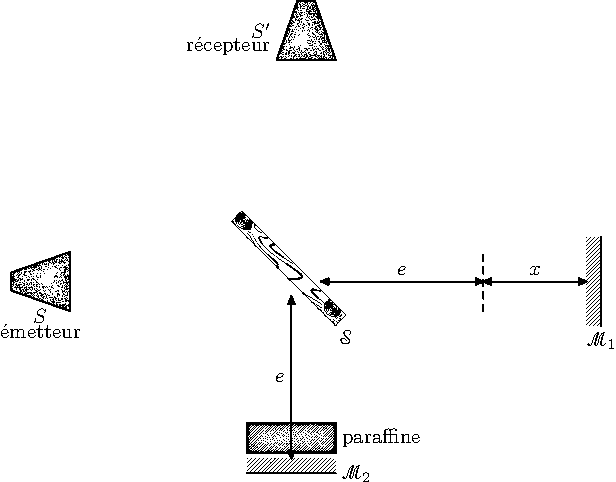
\includegraphics[width=\linewidth]{figures/michelson-2.pdf}
		\caption{Interféromètre de \textsc{Michelson} à onde centimétriques, avec bloc de paraffine}
		\label{fig:montage-paraffine}
	\end{figure}

	On cherche, à présent, à calculer l'indice optique de la paraffine.
	Pour cela, on dispose un bloc de paraffine d'épaisseur \res{$\ell = 19{,}6\:\mathrm{mm}$} accolé au miroir $\mathcal{M}_2$ de l'interféromètre.
	On représente le montage sur la figure~\ref{fig:montage-paraffine}.
	La différence de marche $\delta(x)$ est modifiée par l'ajout de ce bloc de paraffine et, avec les notations de la figure~\ref{fig:montage-paraffine}, on a
	\begin{align*}
		\delta(x) / 2 &= \big((SS')_{\mathrm{voie\ 1}} - (SS')_{\mathrm{voie\ 2}}\big) / 2\\
		&= n_\mathrm{air} e - (e + x - \ell) n_\mathrm{air}  - \ell n_\mathrm{paraffine} \\
		&= x n_\mathrm{air}  + \ell(n_\mathrm{air} - n _\mathrm{paraffine}). \\
	\end{align*}
	On commence par placer les deux miroirs $\mathcal{M}_1$ et $\mathcal{M}_2$ équidistants de $\mathcal{S}$, la séparatrice.
	Ainsi, la différence de marche est donc \[
		\delta(x=0) = \ell (n_\mathrm{air} - n_\mathrm{paraffine}) < 0
	,\] car $n_\mathrm{paraffine} > n_\mathrm{air}$.
	On augmente le déplacement $x$, ainsi $\delta(x)$ augmente également.
	On cherche la valeur de $x$, où $\delta(x)$ serait nul.
	On peut repérer ce déplacement, car l'intensité sera alors maximale.
	Or, lorsque $\delta(x) = 0$, on a \[
		\ell\, n_\mathrm{paraffine}  = n_\mathrm{air} (x + \ell),
	\]d'où, \[
		n_\mathrm{paraffine} = n_\mathrm{air} \cdot \frac{x + \ell}{\ell}
	.\]

	On réalise le protocole décrit précédemment, et on trouve \res{$x = 7\:\mathrm{mm}$}. On en déduit donc que \res{$n_\mathrm{paraffine} = 1{,}4$}, ce qui correspond avec les valeurs connues.

	Finalement, on décide de mesurer la vitesse $v_0$ d'une voiture-jouet sur laquelle on a fixé une plaque métallique.
	On reprend le montage de la figure~\ref{fig:montage-michelson}, mais le miroir $\mathcal{M}_1$ est placé sur la voiture.
	En considérant $x$, le déplacement de la voiture, on en déduit l'expression de la différence de marche : \[
		\delta(x) = 2x n_\mathrm{air} 
	,\] car on a réalisé un interféromètre de \textsc{Michelson} en lame d'air.
	De plus, d'après la formule de \textsc{Fresnel}, on a \[
		I(x) = 2I_0\big(1 + \cos(2\pi\,n_\mathrm{air}\:2x / \lambda_0)\big)
	.\]
	L'intensité $I(x)$ est $(\lambda_0 / 2n_\mathrm{air})$-périodique.
	On lance la voiture-jouet, et on mesure l'intensité $I$ au cours du temps.
	À chaque instant $t$, le déplacement de la voiture est $x = v_0 t$.
	Ainsi, en analysant la période $T$ de $I(t)$, on peut en déduire la vitesse $v_0$ de la voiture : \[
		T = \frac{\lambda_0}{n_\mathrm{air}v_0} \quad\quad\text{ d'où }\quad\quad v_0 = \frac{\lambda_0}{2n_\mathrm{air}  T}
	.\]

	On réalise le protocole décrit précédemment en mesurant, à l oscilloscope, la valeur de $I(t)$.
	On mesure une période de \res{$48{,}62\:\mathrm{ms}$}, et donc \res{$v_0 = 32{,}50\:\mathrm{cm}/\mathrm{s}$}.

	\centerline{\pgfornament[width=3cm]{88}}

	La mesure d'un indice optique d'un matériau peut être réalisée avec un montage bien plus simple à mettre en place qu'un interféromètre de \textsc{Michelson} pour la lumière visible.
	Cependant, les mesures réalisées sont moins précises.
	
	La mesure de vitesse est cependant plus précise avec un Michelson à ondes centimétriques : la longueur d'onde est la seule distance à connaître, et le temps de réaction de l'expérimentateur n'apparaît pas.

	Un interféromètre de \textsc{Michelson} à ondes centimétriques est donc bien utile pour obtenir des valeurs relativement précises.


	\sign

	~
\end{document}
